\documentclass[12pt,english]{article}
\usepackage{fullpage,enumitem,amsmath,amssymb,graphicx}

% Some macros for your convenience
\newcommand\bbR{\ensuremath{\mathbb{R}}} % Real numbers
\newcommand\bbZ{\ensuremath{\mathbb{Z}}} % Integers
\newcommand\bbE{\ensuremath{\mathbb{E}}} % Expectation
\DeclareMathOperator*{\tr}{tr} % Trace
\DeclareMathOperator*{\diag}{diag} % Diagonal matrix
\DeclareMathOperator*{\sign}{sign} % Sign
\DeclareMathOperator*{\var}{Var} % Variance
\DeclareMathOperator*{\cov}{Cov} % Covariance
\newcommand{\1}{\mathbb{I}} % Indicator 

\title{
{\large CS229T/STATS231 Winter 2014 -- Project Progress Report }
}

\author{ \large
Awni Hannun \\
\texttt{awni@stanford.edu}
\and
Peng Qi \\
\texttt{pengqi@stanford.edu}
}
\date{}

\begin{document}
\maketitle

\subsubsection*{Introduction}
We attempt to prescribe a stochastic optimization procedure for the typical
multilayer neural network objective. We plan to do this by developing a deeper
understanding of the most common objective(s) and architectures used in this
setting. We apply this analysis to motivate the selection of optimization
procedures we study and attempt to give a thorough comparison of a few
competing algorithms using existing theory and empirical results. 

\subsubsection*{Experimental Setup}

In most experiments performed, we use a standard multilayer neural network with
dense connections between each layer of hidden activations. The number of
hidden layers and size of the networks vary; for the MNIST experiments
described below we use 2 hidden layers with 200 units each. The leaky rectified
linear nonlinearity ($f(x) = \max\{0.01x,x\}$) is applied at each hidden unit.
Most computation is accelerated using GPUs and the Gnumpy library for Python. 

We use the MNIST handwritten digits dataset which consists of 60,000 training
images and 10,000 test images. The images are all $28\times28$ pixels; however,
prior to training most networks we project the data onto the leading principal
components (between 50 and 100) with standard PCA and use this as the input.
This primarily achieves computational efficiency by decreasing the total number
of parameters in the network. 

\subsubsection*{Understanding the Objective}

In order to gain insight into the objective function landscape of neural
networks in terms of their parameters, we ran a set of experiments with neural
network models that are comparatively smaller than those used in our
optimization experiments.  Specifically, the networks we used have an input
dimension of 50, an output dimension of 10 (determined by the classification
task), and hidden layers with 16 units for each layer. We try to limit the
model size in order to a) efficiently train the networks for repeated runs, and
b) to save the trace of model parameters as well as gradients as the training
progresses to visualize the cost function landscape.

As we train these small networks with SGD, we vary the number of hidden layers
from zero to five, as well as the minibatch size in $\{120,600,6000,60000\}$.
While adding hidden layers is known to help increase the expressivity of the
model, we attempt to investigate if more layers also makes the objective
function of the network more poorly conditioned. Further we wish to know how
good of an approximation to the objective function of the network we have as
function of the minibatch size.

For each model and minibatch setting, we run SGD for 1,000 iterations with a
fixed learning rate of 0.1, saving at each iteration the parameters of the
network, the objective and gradient evaluated for that minibatch. For each
model/minibatch setting, we repeat the network training from 20 independent
random initializations and plot these training traces with a technique
introduced below on the same plot to visualize the landscape of cost function.
For the largest model that we considered in this analysis (5 hidden layers of
16 units each) our trace files will take tens of megabytes on disk, thus we are
constrained to consider small modelsizes.

With these traces, we visualize the cost functions by linear projections to a
lower dimensional space. Specifically, we compute the principal components of
the covariance matrix of the gradient traces across the 20 trials for each
setting, and project the model parameters into the subspace of the leading
principle values. The logic behind this is that we want to characterize the
landscape of the cost function in the direction where the model parameters
(despite initialization) travel the most \footnote{An tempting alternative
would be to project the parameters into the space of the principal components
of the parameter's covariance, but this essentially contradicts our purpose,
and yields uninteresting results that we choose not to show.}. However, despite
our earlier success in visualization with small random perturbations to the
same initialization points, this does not appear to be the case for general
random initializations (See Figure \ref{fig:cost_layer} and
\ref{fig:cost_minibatch}).

Although the visualization does not convey much information beyond models with more
than zero hidden layers (which is essentially softmax regression model, which has a
convex cost function), but from Figure \ref{fig:cost_layer} we do get a rough sense 
that the nolinearity of the cost function of neural networks grows as the number
of hidden layer increases. We can see that the random initialization points (red end
for each trace) are more concentrated under linear projection
for the shallow models than for the deep ones. Another interesting phenomenon is that
as the size of minibatch shrinks, the minibatch cost function landscape deviates further
from the batch cost function (Figure \ref{fig:cost_minibatch}), and this might worth
investigating in our further analyses as this might characterize the non-stationarity
of neural network cost functions on minibatches.

\section{Optimization}

We consider two families of stochastic optimization algorithms. Traditionally
used in optimizing deep neural networks, the first class is that of momentum
based methods which have recently been generalized and included the broader
group of accelerated gradient algorithms \cite{sutskever_2013}. The second class
includes variations on the adaptive gradient algorithms as presented in
\cite{duchi_2011}.

\subsection{Accelerated Gradient}

The accelerated gradient methods are a generalization of the basic stochastic
gradient descent (SGD) optimization procedure. Let $\ell(\theta)$ be the loss
function of the network with parameters $\theta$. We use accelerated SGD
methods that update the parameters at time $t$ according to
\begin{equation}
\label{nag}
\begin{aligned}
&v_{t+1} = \mu v_t - \eta \nabla \ell (\theta_t + \gamma v_t) \\
&\theta_{t+1} = \theta_t + v_{t+1}
\end{aligned}
\end{equation}
where $\eta$ is the learning rate, and the parameter $\mu$, known as the
momentum parameter, dictates how much gradient history we take into account at
every update. If we set $\mu = 0$ we recover plain SGD, and setting $\mu = 1$
uses the full gradient history at every update.  The $\gamma$ parameter is
either active and set as $\gamma = \mu$ or inactive and set as $\gamma = 0$.
When $\gamma$ is inactive, we have typical SGD with ``momentum'', also known as
classical momentum (CM). On the other hand, when $\gamma$ is active the
procedure is known as Nesterov's accelerated graient (NAG).

A common belief is that network objectives likely suffer from long narrow
ravines leading towards local optima surrounded with walls of high curvature.
This hypothesis motivates the use of momentum to encourage persistent
directions of travel along the basin and suppress unwanted oscillation.

\subsection{Adaptive Gradient}
\label{adagrad}

We study modifications to the adaptive gradient algorithm (AdaGrad) with the
diagonal preconditioning matrix $G$. The update can be written as
\begin{equation}
\begin{aligned}
&G_{t+1} = G_{t} + \diag(\nabla \ell (\theta_t))^2 \\
&\theta_{t+1} = \theta_t - G_{t+1}^{-1/2} \nabla \ell(\theta_t)
\end{aligned} 
\end{equation}

In some sense AdaGrad achieves a similar affect as NAG by penalizing
oscillating directions in which we take large steps and encouraging directions
with small but consistent gradients. However, in other aspects the optimization
routines behave quite differently. A simple property of AdaGrad which as we
show later can drasitcally affect optimization is the nondecreasing
monotinicity of the matrix $G$. This leads AdaGrad to penalize large yet
consistent directions of travel in the optimization process. This proves
locally favorable in most of the models studied in the next section, but
globally the behaviour results in better performance of NAG routine over the
vanilla AdaGrad algorithm.

This motivates two simple variations of the AdaGrad algorithm. The first is to
replace the square root on the matrix $G_t$ with a function which grows less
quickly (e.g. cube root). The second is to decay $G_t$ by a factor of $\gamma
\in (0,1]$ before including it in the update for $G_{t+1}$. This is close to
the AdaDelta algorithm presented in \cite{zeiler_2012}, but there they take a
convex combination of the two terms in the update of $G_{t+1}$ whereas here we
only decay the gradient history term.

% Discuss convergence properties of each method?


\subsubsection*{Plans}

Further plans for our project include:

\begin{enumerate}

\item Use alternative dimensionality reduction techniques for cost function
landscape visualization, e.g. t-SNE.

\item Evaluate the same empirical studies on a slightly harder to fit (``more realistic'') dataset.
We plan to move to CIFAR-100 next.

\item Compare the NAG, AdaGrad and other variations of the two optimization
procedures to convergence rates given in the literature.

\item Gain better understanding of the network objective(s) by using second
order information.  For example for small $n$, we can estimate rank $n$
approximations to the Hessian of the objective to better understand local
curvature, and hopefully improve existing algorithms by utilizing
such information.

\item Give an evaluation and discussion on generalization performance.

\end{enumerate}

\newpage
\subsubsection*{Appendix}

\begin{figure}[h!]
{\centering
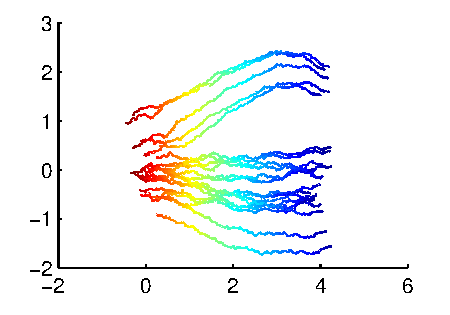
\includegraphics[width=.23\textwidth]{../plots/results_.pdf} 
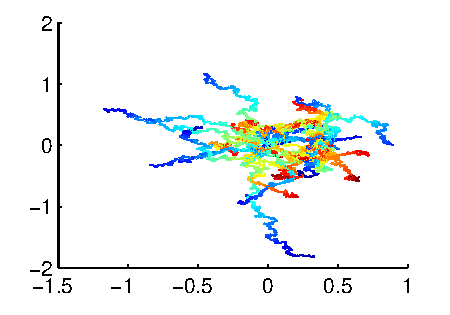
\includegraphics[width=.23\textwidth]{../plots/results_16.pdf} 
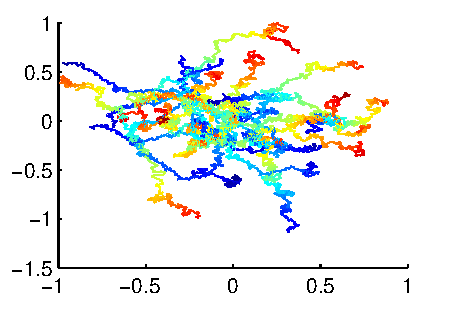
\includegraphics[width=.23\textwidth]{../plots/results_16_16.pdf}
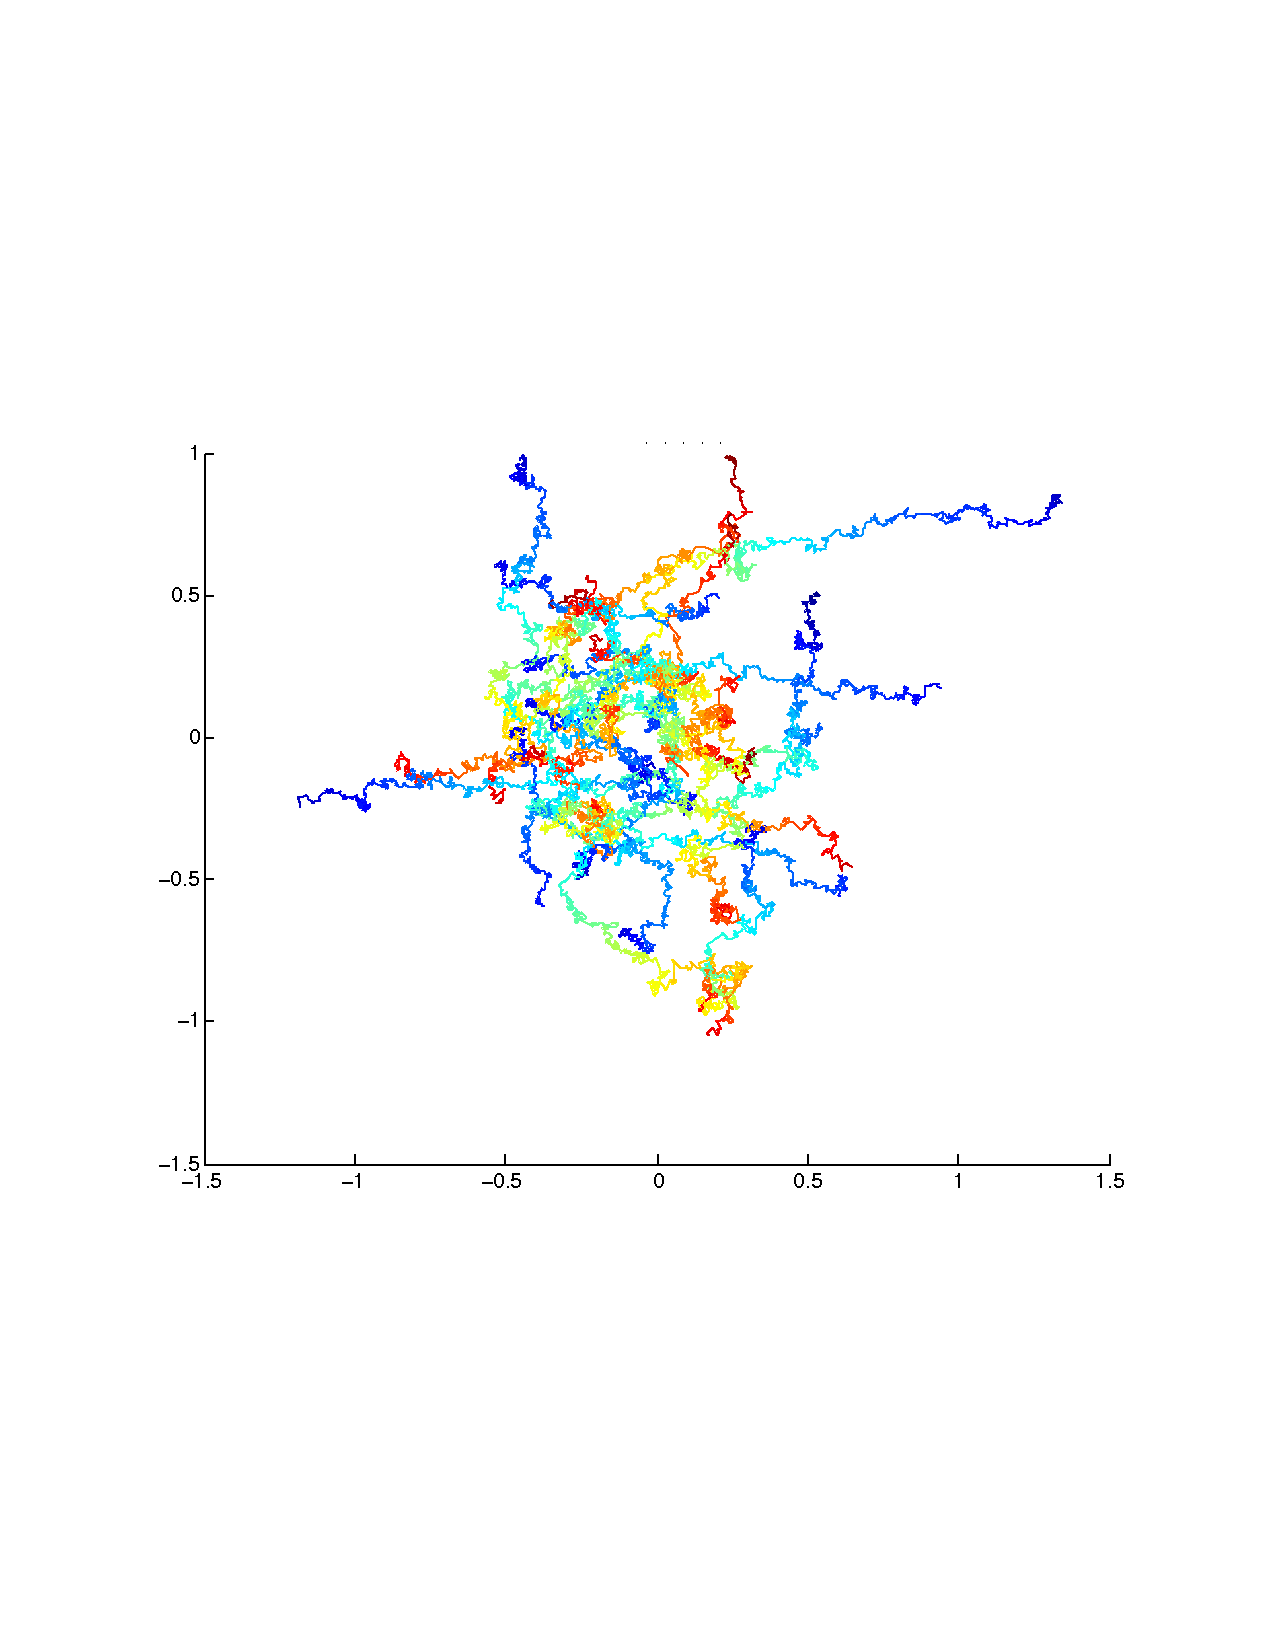
\includegraphics[width=.23\textwidth]{../plots/results_16_16_16_16_16.pdf}
}
\caption{Visualization of cost function landscapes for neural networks of hidden layer number 0, 1, 2, and 5} \label{fig:cost_layer}
\end{figure}

\begin{figure}[h!]
{\centering
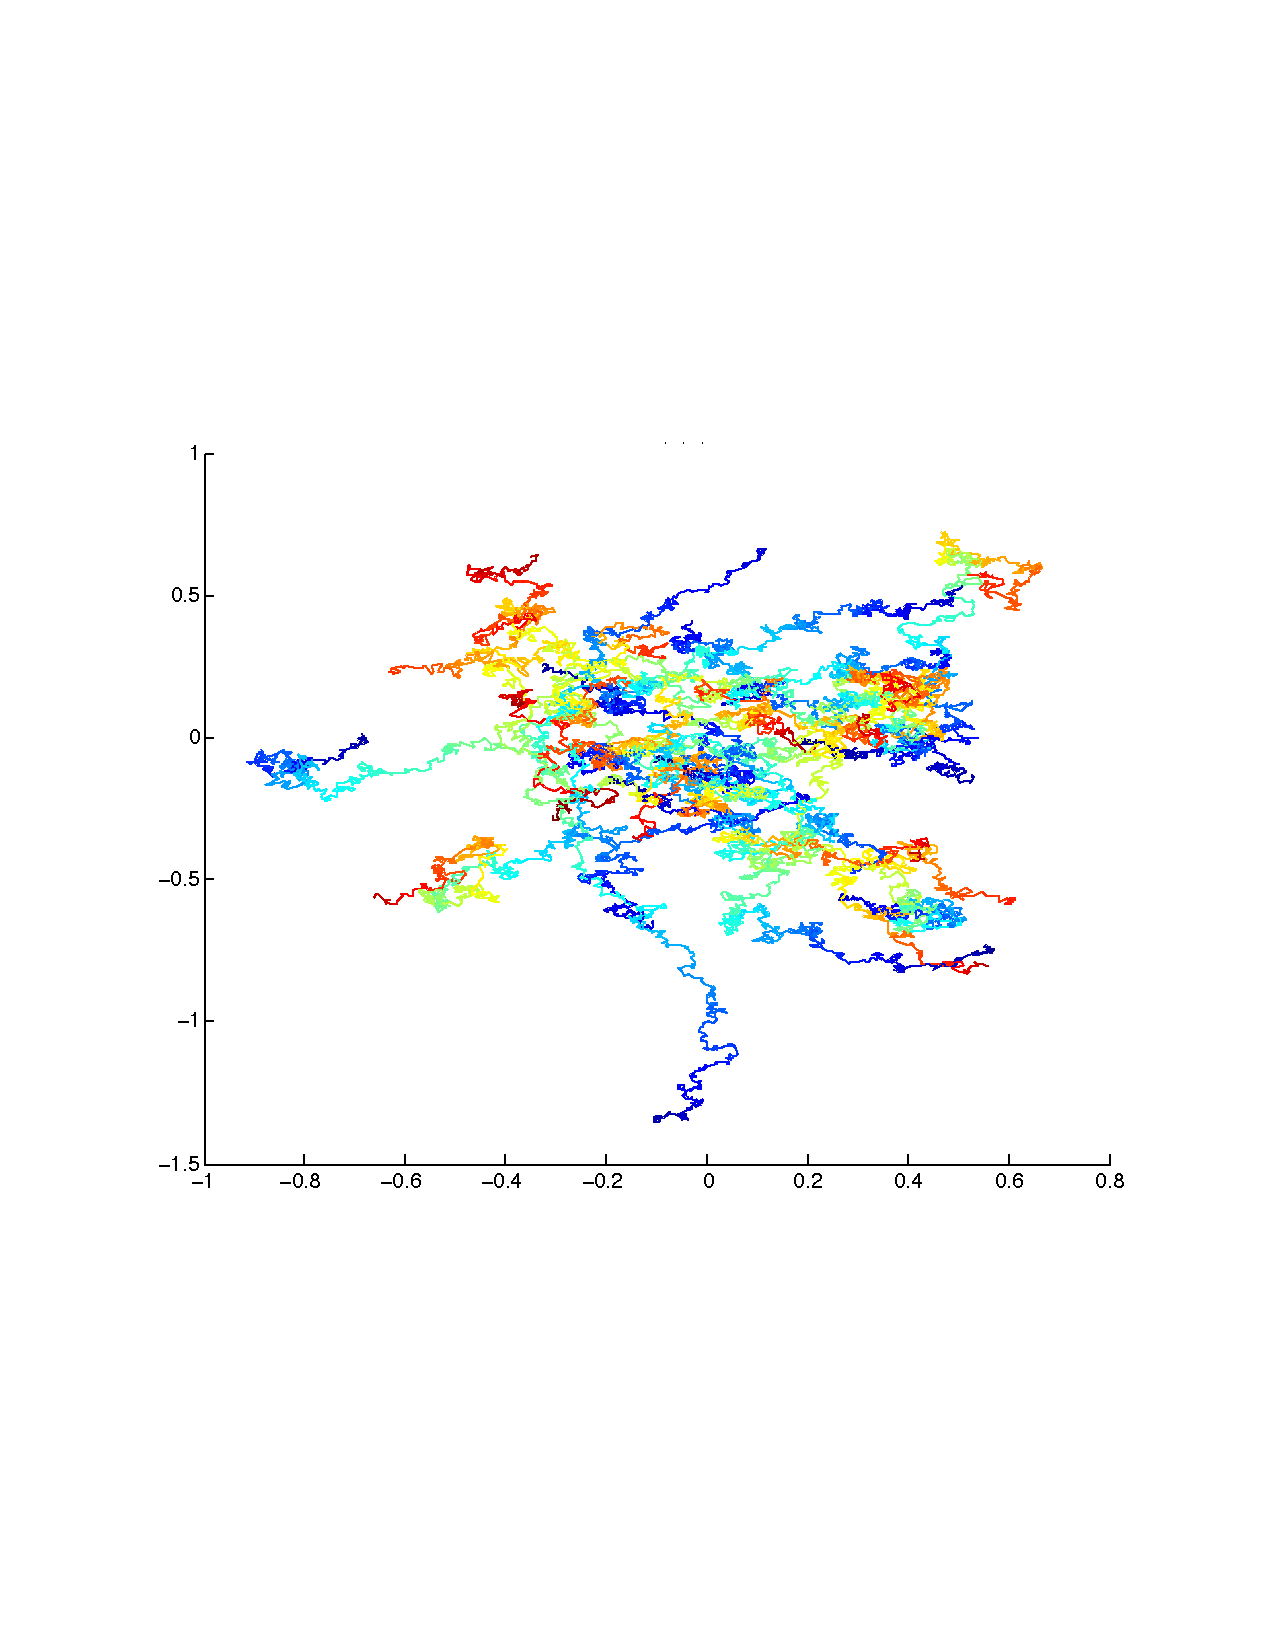
\includegraphics[width=.23\textwidth]{../plots/results_16_16_16.pdf}
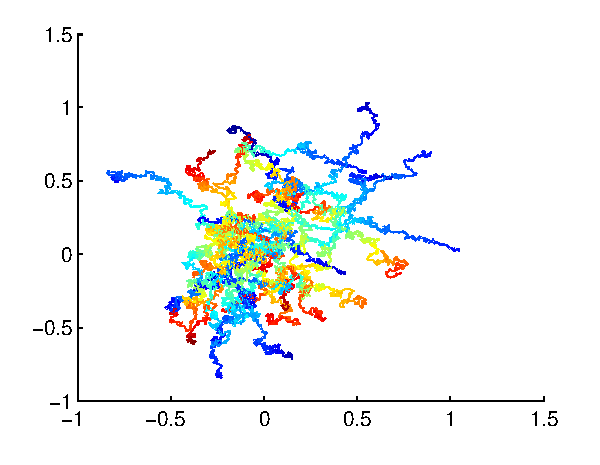
\includegraphics[width=.23\textwidth]{../plots/results_[6000]_16_16_16.pdf}
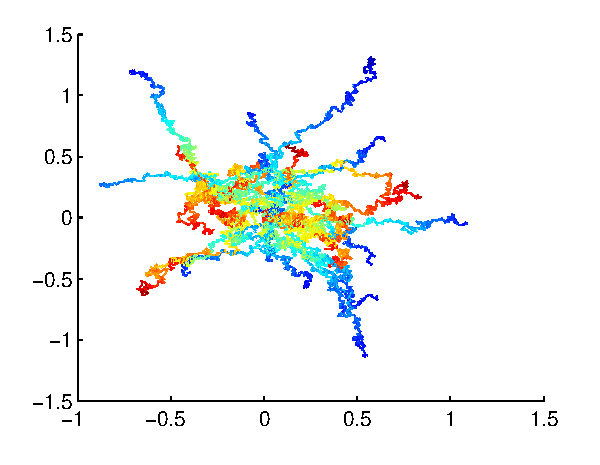
\includegraphics[width=.23\textwidth]{../plots/results_[600]_16_16_16.pdf}
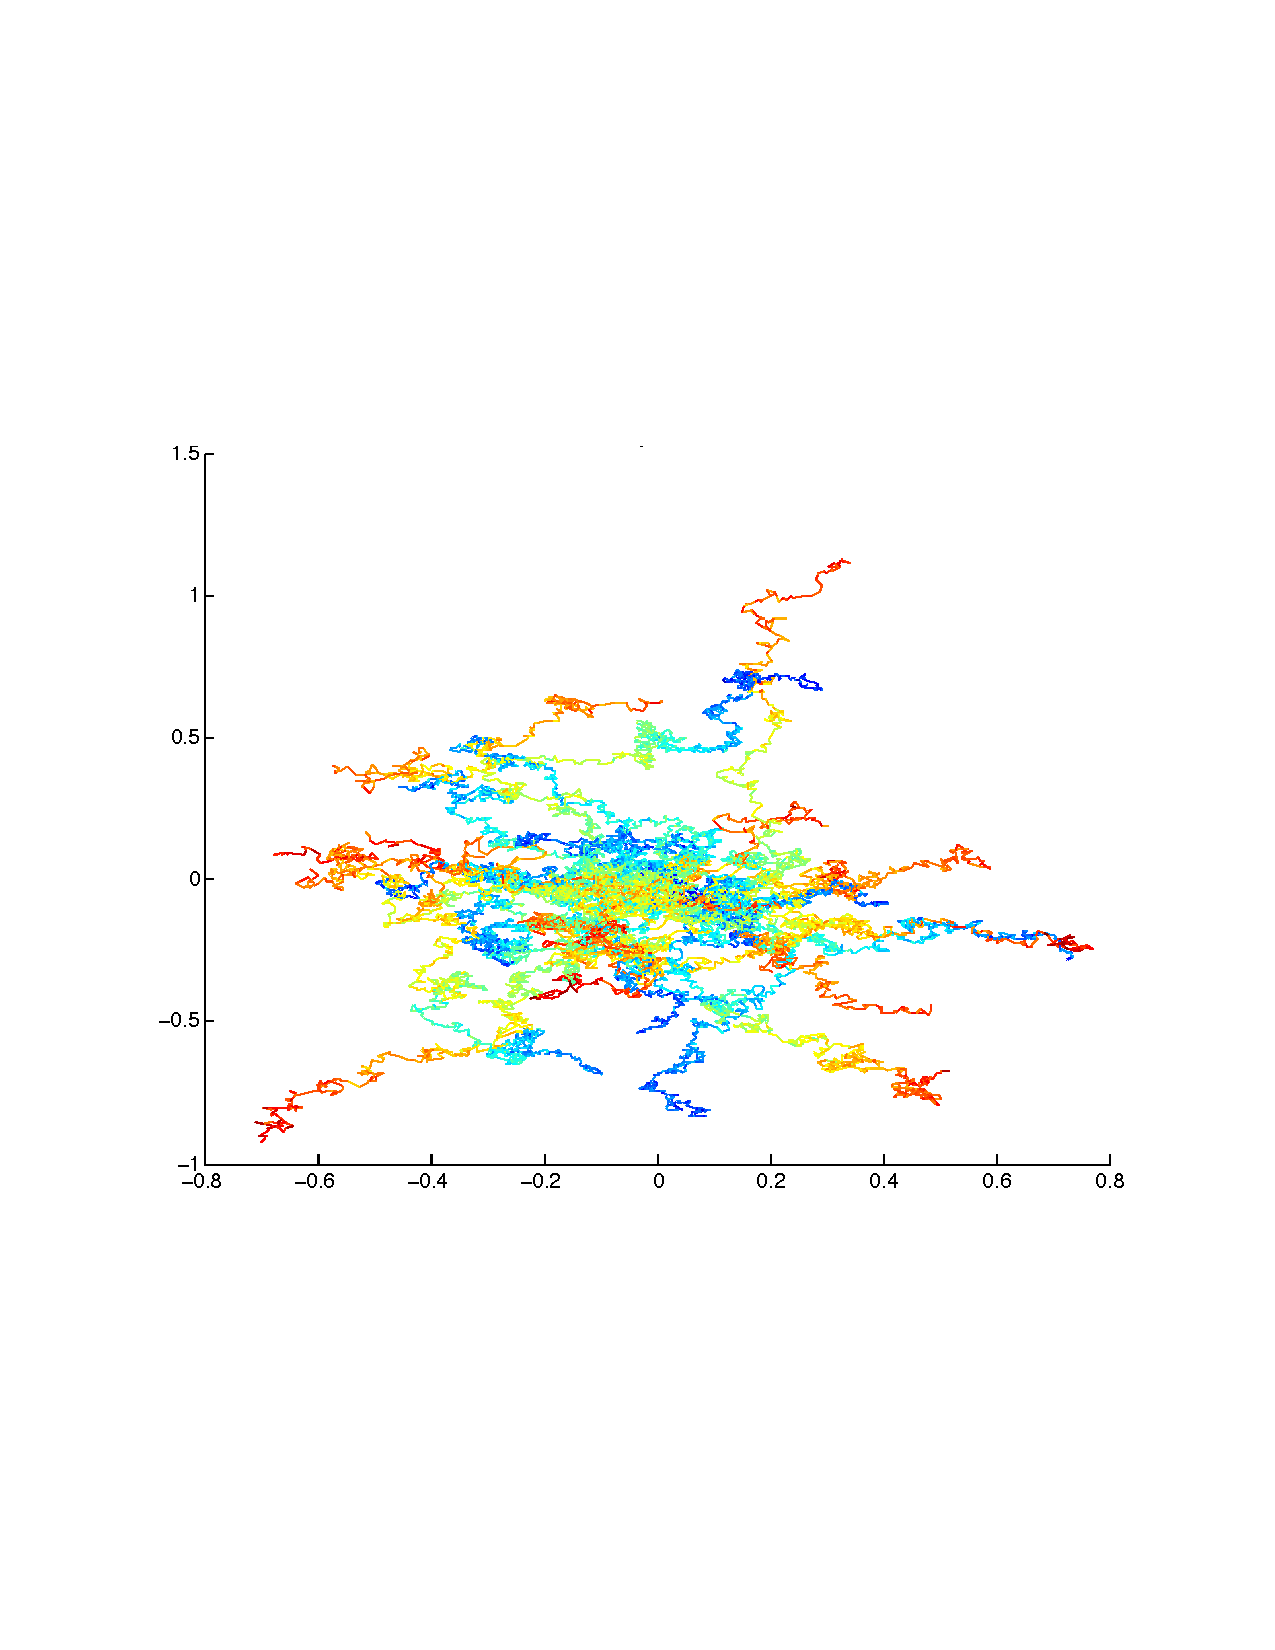
\includegraphics[width=.23\textwidth]{../plots/results_[120]_16_16_16.pdf}
}
\caption{Visualization of cost function landscapes for neural networks of 3 hidden layers, trained with minibatche sizes 60000, 6000, 600, and 120}\label{fig:cost_minibatch}
\end{figure}

\begin{figure}[h!]
    \centering
    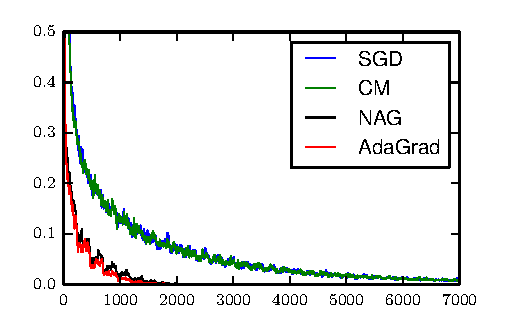
\includegraphics{../plots/allcurves.pdf}
    \caption{\label{fig:allcurves} Plot of estimated objective on the training
set over iterations of optimization.}
\end{figure}

\begin{figure}[h!]
    \centering
    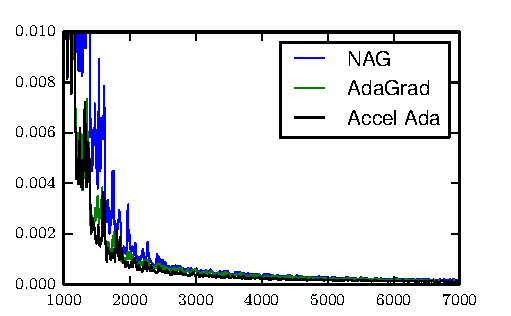
\includegraphics{../plots/bestcurves.pdf}
    \caption{\label{fig:bestcurves} Plot of estimated objective with scaled
y-axis in order to see finer differences between the three best optimization
methods.}
\end{figure}

\bibliography{refs}{}
\bibliographystyle{plain}

\end{document}

